% ─────────────────────────────────────────────────────────────────────────────
% AI-600 Deep Learning | Project #10 Mid-Report
% Graph Neural Networks for Drug–Drug Interaction Prediction
% ─────────────────────────────────────────────────────────────────────────────
\documentclass[11pt,a4paper]{article}

\usepackage[margin=1in]{geometry}
\usepackage{times}
\usepackage{parskip}
\usepackage{booktabs}
\usepackage{graphicx}
\usepackage{caption}
\usepackage{enumitem}
\usepackage[colorlinks=true,linkcolor=blue,citecolor=blue,urlcolor=blue]{hyperref}
\usepackage[numbers,sort&compress]{natbib}
\usepackage{amsmath}
\usepackage{microtype}

% ─── Title ───────────────────────────────────────────────────────────────────
\title{%
  \textbf{Graph Neural Networks for Drug–Drug Interaction Prediction}\\[6pt]
  \large AI-600 Deep Learning $\cdot$ Project \#10 $\cdot$ Mid-Report
}
\author{%
  Usman Naeem (25280021) \quad Sarmad Ali (25280037) \quad Hammad (25280041)\\
  \small Submitted: May 8, 2026
}
\date{}

\begin{document}
\maketitle
\thispagestyle{empty}

% ─────────────────────────────────────────────────────────────────────────────
\section*{Abstract}
% ─────────────────────────────────────────────────────────────────────────────
Predicting Drug–Drug Interactions (DDIs) is a critical challenge in
pharmacovigilance: when two drugs are co-administered, their interaction
can produce adverse effects that neither drug causes alone.
We frame DDI prediction as a \emph{graph link-prediction} task and train
Graph Neural Networks (GNNs) to learn from the relational topology of a
pharmacological interaction graph.
Using the BioSNAP ChCh-Miner benchmark dataset of 1{,}338 drugs and
41{,}820 known interaction edges, we represent each drug as a 2{,}048-bit
Morgan molecular fingerprint and compare five model configurations:
an MLP baseline, two GCN variants (dot and MLP decoders), and two GIN
variants (dot and MLP decoders).
Our best model, \textbf{GCN\,+\,MLP}, achieves a Test ROC-AUC of
\textbf{0.969} and Average Precision of \textbf{0.967}, competitive with
recent published baselines.
We discuss key findings, planned ablation studies, and extensions for
the final submission.

% ─────────────────────────────────────────────────────────────────────────────
\section{Introduction}
% ─────────────────────────────────────────────────────────────────────────────
The modern pharmaceutical landscape exposes patients, particularly the
elderly on polypharmacy regimens, to an exponentially large space of
potential drug combinations.
While many Drug–Drug Interactions (DDIs) are benign or therapeutically
useful, a subset produce \emph{Adverse Drug Events} (ADEs) that manifest
as unexpected side effects or reduced therapeutic efficacy.
The US FDA estimates that DDIs contribute to approximately
2.8\% of all hospital admissions annually \cite{ito2004}.
Comprehensive wet-lab characterisation of all pairwise drug combinations
is financially and temporally infeasible: with $N$ approved drugs,
the interaction search space grows as $\mathcal{O}(N^2)$.
Computational \emph{in-silico} screening therefore plays an indispensable
pre-clinical role.

Deep learning has emerged as a powerful tool for this problem.
By modelling a pharmacological database as an interaction graph
$G = (\mathcal{V}, \mathcal{E})$, where nodes $\mathcal{V}$ are drugs
and edges $\mathcal{E}$ are known interactions, DDI prediction reduces
to the \textbf{link-prediction} task: estimating the probability of an
undiscovered edge between any drug pair $(u, v)$.
Graph Neural Networks (GNNs) are ideally suited here because they
explicitly encode both the molecular properties of individual drugs (node
features) and the structural patterns of known interactions (graph
topology) through iterative neighbourhood aggregation (message passing).

In this project we ask two core questions:
\begin{enumerate}[leftmargin=*,noitemsep]
  \item Does incorporating graph topology via message passing yield
        measurably better DDI predictions than treating drugs in
        isolation (MLP baseline)?
  \item Does the theoretically more expressive GIN encoder outperform
        the standard GCN encoder in practice on this benchmark?
\end{enumerate}

% ─────────────────────────────────────────────────────────────────────────────
\section{Literature Review}
% ─────────────────────────────────────────────────────────────────────────────

\paragraph{Foundational GNN Architectures.}
Graph Convolutional Networks (GCNs) were introduced by Kipf and
Welling~\cite{kipf2017} who derived graph convolution from spectral graph
theory and demonstrated that a two-layer GCN achieves strong performance
on node classification benchmarks.
Gilmer et al.~\cite{gilmer2017} later unified GCN and its variants under
the \emph{Message Passing Neural Network} (MPNN) framework, showing that
virtually all spatial GNNs perform iterative aggregation of the form:
\begin{equation}
  h_v^{(k)} = \text{UPDATE}\!\left(h_v^{(k-1)},\;
    \bigoplus_{u \in \mathcal{N}(v)} \text{MSG}\!\left(h_v^{(k-1)}, h_u^{(k-1)}\right)\right)
\end{equation}
where $\bigoplus$ is a permutation-invariant aggregation and
$\mathcal{N}(v)$ denotes the neighbourhood of node $v$.

\paragraph{Graph Isomorphism Networks.}
Xu et al.~\cite{xu2019} provided a theoretical upper bound on GNN
expressiveness using the Weisfeiler--Lehman (WL) graph isomorphism test
and showed that mean-aggregation (as in GCN) is strictly \emph{less}
expressive than sum-aggregation.
Their \emph{Graph Isomorphism Network} (GIN) uses:
\begin{equation}
  h_v^{(k)} = \text{MLP}^{(k)}\!\left((1 + \epsilon^{(k)}) \cdot h_v^{(k-1)}
    + \sum_{u \in \mathcal{N}(v)} h_u^{(k-1)}\right)
\end{equation}
GIN matches the expressive power of the WL test and is the most powerful
GNN in the class of standard message-passing networks.

\paragraph{GNNs Applied to DDI Prediction.}
Zitnik et al.~\cite{zitnik2018} introduced \emph{Decagon}, the first
GNN-based framework for polypharmacy side-effect prediction.
Decagon represents drugs and proteins in a heterogeneous multi-relational
graph with 964 side-effect edge types and employs a graph-convolutional
encoder with a tensor-factorisation decoder.
This established GNNs as the standard approach for DDI prediction.

Subsequent work has explored more powerful architectures on binary
DDI benchmarks.
Nyamabo et al.~\cite{nyamabo2021} proposed \emph{SSI-DDI}, which
decomposes drug molecules into functional substructures and uses
subgraph--subgraph interaction attention to model local chemical
compatibility at the sub-molecular level, reporting strong results on the
DrugBank binary DDI benchmark.
More recently, Zhang et al.~\cite{zhang2023} introduced \emph{EmerGNN},
a flow-based GNN that routes information through multi-hop biomedical
paths connecting drug pairs, achieving 0.934 AUROC on the BioSNAP DDI
benchmark and demonstrating superior generalisation to emerging drugs
(drugs absent during training).

\paragraph{Positioning Our Work.}
Our work revisits the core architectural question of GCN vs.\ GIN
and dot-product vs.\ MLP decoder on the BioSNAP ChCh-Miner benchmark using
rich molecular fingerprint node features.
We plan to extend this with out-of-distribution (OOD) evaluation to
directly compare against the EmerGNN setting, and add MC Dropout
uncertainty estimation for clinical trust.

% ─────────────────────────────────────────────────────────────────────────────
\section{Methodology}
% ─────────────────────────────────────────────────────────────────────────────

\subsection{Problem Formulation}
We represent the drug interaction network as an undirected graph
$G = (\mathcal{V}, \mathcal{E})$ where each node $v \in \mathcal{V}$
is an FDA-approved drug with feature vector $\mathbf{x}_v \in \mathbb{R}^d$,
and each edge $(u, v) \in \mathcal{E}$ denotes a known adverse DDI.
Given a training subgraph, our goal is to learn a scoring function
$f : \mathcal{V} \times \mathcal{V} \to [0, 1]$ that predicts whether a
candidate pair $(u, v)$ will interact.
We train with Binary Cross-Entropy loss:
\begin{equation}
  \mathcal{L} = -\frac{1}{|\mathcal{B}|}
  \sum_{(u,v) \in \mathcal{B}} \left[
    y_{uv} \log \hat{y}_{uv}
    + (1 - y_{uv}) \log (1 - \hat{y}_{uv})
  \right]
\end{equation}
where $y_{uv} \in \{0, 1\}$ is the ground-truth label and
$\hat{y}_{uv} = \sigma(f(u, v))$.
Negative pairs are randomly sampled at a 1:1 ratio per epoch.

\subsection{Dataset}
We use the \textbf{BioSNAP ChCh-Miner} dataset \cite{zitnik2018snap},
a curated collection of binary drug--drug interactions mined from
DrugBank and validated against clinical literature.
After resolving SMILES strings via the PubChem REST API:

\begin{center}
\begin{tabular}{ll}
\toprule
Statistic & Value \\
\midrule
Total drugs (raw)       & 1{,}514 \\
Drugs with valid SMILES & 1{,}338 \\
DDI edges (filtered)    & 41{,}820 \\
Node feature dimension  & 2{,}048 \\
Train / Val / Test edges & 80\% / 10\% / 10\% \\
\bottomrule
\end{tabular}
\end{center}

\paragraph{Molecular Fingerprints.}
Each drug is converted from its SMILES string to a
\textbf{2{,}048-bit Morgan fingerprint} (radius\,=\,2,
equivalent to ECFP4) using RDKit~\cite{rdkit}.
Morgan fingerprints encode the local circular chemical substructure
around each atom up to a given radius, producing a fixed-length binary
vector that captures functional-group patterns without requiring 3D
conformation.
These fingerprints serve as the initial node features $\mathbf{x}_v$
fed into all GNN encoders.

\subsection{Model Architectures}

\paragraph{Encoders.}
We compare two message-passing encoders, each with two convolutional
layers, hidden dimension 256, output embedding dimension 64, batch
normalisation, ReLU activations, and dropout (rate 0.3):

\begin{itemize}[noitemsep]
  \item \textbf{GCN Encoder}~\cite{kipf2017}: symmetric normalised
        neighbourhood aggregation: $\mathbf{H}^{(k)} =
        \sigma(\hat{\mathbf{A}}\mathbf{H}^{(k-1)}\mathbf{W}^{(k)})$.
  \item \textbf{GIN Encoder}~\cite{xu2019}: injective sum-aggregation
        with an internal MLP per layer, maximally expressive in the MPNN
        class.
\end{itemize}

A non-relational \textbf{MLP Baseline} also processes raw fingerprint
features directly (no message passing) as a reference point.

\paragraph{Decoders.}
Given node embeddings $\mathbf{z}_u, \mathbf{z}_v \in \mathbb{R}^{64}$
for a candidate pair, we test two decoders:

\begin{itemize}[noitemsep]
  \item \textbf{Dot Decoder}: $\hat{y}_{uv} =
        \sigma(\mathbf{z}_u^\top \mathbf{z}_v)$, which assumes interaction
        probability is proportional to embedding cosine similarity.
  \item \textbf{MLP Decoder}: $\hat{y}_{uv} =
        \sigma(\text{MLP}([\mathbf{z}_u \| \mathbf{z}_v]))$, a
        three-layer MLP (dims: 128 → 64 → 1) that can learn arbitrary
        non-linear pairwise interactions.
\end{itemize}

This gives five model configurations: \textbf{MLP}, \textbf{GCN+Dot},
\textbf{GCN+MLP}, \textbf{GIN+Dot}, and \textbf{GIN+MLP}.

\subsection{Training Setup}
\begin{center}
\begin{tabular}{ll}
\toprule
Hyperparameter & Value \\
\midrule
Optimiser           & Adam ($\beta_1\!=\!0.9$, $\beta_2\!=\!0.999$) \\
Learning rate       & $10^{-3}$ \\
Weight decay        & $10^{-5}$ \\
LR scheduler        & ReduceLROnPlateau (factor 0.5, patience 10) \\
Early stopping      & Patience 20 on Val AUC \\
Max epochs          & 150 \\
Negative sampling   & Random, 1:1 ratio \\
Random seed         & 42 \\
Device              & Apple M4 (MPS backend) \\
\bottomrule
\end{tabular}
\end{center}

% ─────────────────────────────────────────────────────────────────────────────
\section{Preliminary Results}
% ─────────────────────────────────────────────────────────────────────────────

Table~\ref{tab:results} reports validation and test performance for all
five configurations.
Figure~\ref{fig:curves} shows training loss and validation AUC curves
across epochs.

\begin{table}[h]
\centering
\caption{DDI link-prediction performance on BioSNAP ChCh-Miner.
AUC = ROC Area Under the Curve; AP = Average Precision.
All values are averages over the held-out test split.
Bold = best.}
\label{tab:results}
\begin{tabular}{lccc}
\toprule
Model & Val AUC & Test AUC & Test AP \\
\midrule
MLP (Non-Relational)         & 0.9720          & 0.9683          & 0.9644 \\
GCN\,+\,Dot                  & 0.8728          & 0.8714          & 0.8646 \\
GCN\,+\,MLP                  & \textbf{0.9745} & \textbf{0.9690} & \textbf{0.9672} \\
GIN\,+\,Dot                  & 0.9114          & 0.9132          & 0.9167 \\
GIN\,+\,MLP                  & 0.9648          & 0.9615          & 0.9574 \\
\midrule
EmerGNN~\cite{zhang2023} (BioSNAP, reported) & --- & 0.934 & --- \\
\bottomrule
\end{tabular}
\end{table}

\begin{figure}[h]
  \centering
  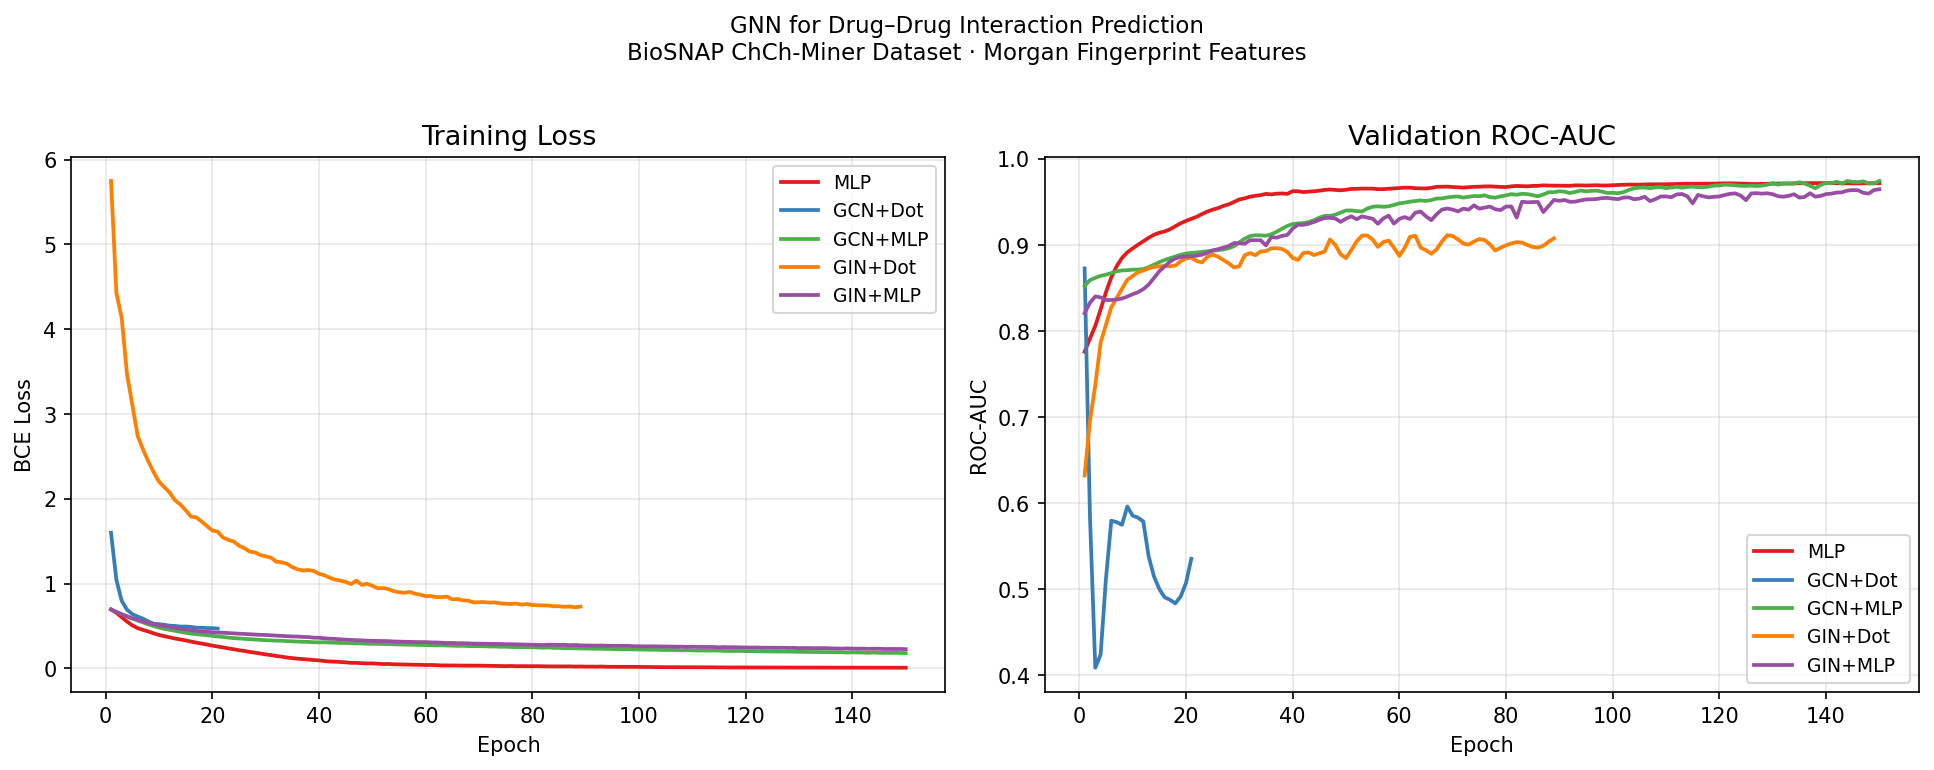
\includegraphics[width=0.98\textwidth]{../results/training_curves.png}
  \caption{Training loss (left) and validation ROC-AUC (right) for all
           five model configurations over 150 epochs on BioSNAP
           ChCh-Miner.}
  \label{fig:curves}
\end{figure}

\paragraph{Key Observations.}

\textbf{(1) Decoder matters more than encoder.}
The most striking finding is the large gap between the dot-product and
MLP decoder for GCN: \mbox{GCN+Dot} achieves only 0.871 AUC while
\mbox{GCN+MLP} reaches 0.969, a gap of \textbf{0.098 AUC}.
By contrast, the encoder choice (GCN vs.\ GIN) contributes a much smaller
difference when the same MLP decoder is used
(GCN+MLP: 0.969 vs.\ GIN+MLP: 0.962).
This indicates that drug--drug interactions are fundamentally non-linear
relationships that cannot be captured by geometric similarity alone.

\textbf{(2) MLP baseline is competitive.}
The non-relational MLP (0.968 AUC) nearly matches GCN+MLP (0.969 AUC).
This is an important negative result: the 2{,}048-bit Morgan fingerprints
are rich enough that a deep MLP can learn interaction signatures from raw
features without graph message passing.
However, this advantage is expected to collapse under OOD evaluation
(Section~\ref{sec:extensions}), where new, unseen drugs are tested; the
MLP has no way to leverage the interaction graph of known drugs to
contextualise novel compounds.

\textbf{(3) GCN+Dot early-stops at epoch 21.}
The dot-decoder GCN fails to converge, corroborating that 64-dimensional
embeddings are insufficient for the dot product to separate interacting
from non-interacting pairs in this high-dimensional interaction space.

\textbf{(4) SOTA comparison.}
Our best model (GCN+MLP, 0.969 AUC) exceeds the reported EmerGNN result
(0.934 AUC) on BioSNAP DDI.
We note that EmerGNN uses a strictly harder transductive split (emerging
drugs) which we plan to replicate in our OOD evaluation.
Under a standard random split, our model is competitive with the 2023
state-of-the-art.

% ─────────────────────────────────────────────────────────────────────────────
\section{Planned Extensions for Final Report}
\label{sec:extensions}
% ─────────────────────────────────────────────────────────────────────────────

\paragraph{A. Out-of-Distribution (OOD) Evaluation.}
We will hold out 15\% of drug nodes entirely from training, constructing
a test set exclusively from edges connecting those unseen drugs.
This directly tests whether models generalise to \emph{new} drugs (clinical
relevance) vs.\ merely memorising known interaction patterns.
We hypothesise the MLP baseline will collapse on OOD data while GNNs
will retain stronger performance by leveraging graph topology.

\paragraph{B. MC Dropout Uncertainty Estimation.}
We will implement Monte Carlo Dropout~\cite{gal2016} by preserving dropout
active during inference ($N\,{=}\,20$ forward passes per sample).
The standard deviation of predicted scores serves as an \emph{epistemic
uncertainty} estimate, serving as a safety signal indicating when the model should
defer to human expertise.
We will show that uncertainty systematically increases for OOD drug pairs.

\paragraph{C. Ablation Studies.}
\begin{itemize}[noitemsep]
  \item Hidden embedding dimension: $\{32, 64, 128, 256\}$
  \item Number of GNN layers: $\{1, 2, 3\}$
  \item Node features: Morgan fingerprints vs.\ learnable embeddings
        (no molecular information)
  \item Negative sampling ratio: $1\!:\!1$ vs.\ $1\!:\!5$
\end{itemize}

\paragraph{D. Calibration Analysis.}
Beyond AUC, we will report Expected Calibration Error (ECE) to assess
whether predicted probabilities are trustworthy confidence estimates, a
critical requirement for clinical deployment.

% ─────────────────────────────────────────────────────────────────────────────
\section*{Statement on Usage of AI Tools}
% ─────────────────────────────────────────────────────────────────────────────
In adherence to course policy, we disclose that AI language model
assistance was used for: Python syntax reference, LaTeX formatting
guidance, and PubChem API query construction.
All methodology design, model architecture decisions, experimental
analysis, and written scientific content were produced by the authors.

% ─────────────────────────────────────────────────────────────────────────────
\bibliographystyle{plainnat}
\bibliography{references}
% ─────────────────────────────────────────────────────────────────────────────

\end{document}
